
\section{Atomic Physics}
(such as proper ties of electrons, Bohr model, energy
quantization, atomic structure, atomic
spectra, selection rules, black-body
radiation, x-rays, atoms in electric and
magnetic fields)


\subsection{Properties of electrons}  
\Table{
\hline
Spin
&
\MiniPg{.7}{
\center
They are fermions, $s=\frac{1}{2}$.
}
\\ \hline
}

%%%%%%%%%%%%%%%%%%%%%%%%%%%%%%%%%%%%%%

\subsection{Bohr Model}  
\Table{
\hline

Derive orbital radius & Classical centripetal force for electron about a nucleus: \\
& $\bold{F} = m\bold{a} \Rightarrow \dfrac{Ze^2}{4 \pi \epsilon_0 \, r^2} = \dfrac{m_ev^2}{r}$ \\
& Orbital momentum is quantized in units of $\hbar$, i.e. $mvr = n\hbar$ \\
& Therefore, $\boxed{ r_n = \dfrac{4 \pi \epsilon_0 \, n^2\hbar^2}{Ze^2 m_e} }$ \\
orbital radius $r(n,Z)$ & $r(n,Z) = \dfrac{n^2 a_0}{Z}$

\\ \hline

Bohr radius &  $a_0 = \dfrac{4 \pi \epsilon_0 \, \hbar^2}{e^2 m_e} = \dfrac{\hbar}{m_e \, c \, \alpha} = 0.53 \, \angst$\\
\& Fine Structure Constant & where $\alpha \approx \dfrac{1}{137}$ is the Fine Structure constant.

\\ \hline

Wave function ground state H

&

$\psi_{1 0 0}(r, \theta, \phi) = \dfrac{1}{\sqrt{\pi a^3}}e^{-r/a} \boxed{\propto e^{-r/a}}$

\\ \hline
}

\Table{
\hline
Binding and Rydberg Energy 

&

$E_B = - \dfrac{1}{4 \pi \epsilon_0} \dfrac{Z e^2}{2 r_n}  = -\dfrac{R_E Z^2}{n^2} $ where $R_E = \dfrac{m_e e^4}{8 \epsilon_0^2 h^2} = 13.6 \textrm{ eV}$

\\ \hline

Positronium binding energy & Positronium is a bound state of an electron and positron \\
& Use formulation as Hydrogen, but with electron reduced mass: \\
& $m_{\textrm{red}} = \dfrac{m_e m_p}{m_e + m_p} = m_e \dfrac{1}{1 + m_e/m_p} = m_e/2$ \\
& So, $E_n = \dfrac{R_E}{2n^2} $ for positronium.

 \\ \hline
}

%%%%%%%%%%%%%%%%%%%%%%%%%%%%%%%%%%%%%%%

\subsection{Energy quantization}
\Table{
\hline

\MiniPg{.4}{

Typical atomic/molecular energy levels by type

}

&

\MiniPg{.6}{
\center

Electronic levels: $\sim$ 1 eV

Vibrational levels: $\sim$ 0.1 eV

Rotational levels: $\sim$ 0.001 eV

}

\\ \hline

Energy of photon emitted by H atom & $E = E_i - E_f = R_E \Big(\dfrac{1}{n_f^2} - \dfrac{1}{n_i^2} \Big)$

\\ \hline

Wavelength of photon & $E = h \nu = \dfrac{hc}{\lambda} $ \\
& Wavelength given by $ \dfrac{1}{\lambda} = R \Big(\dfrac{1}{n_f^2} - \dfrac{1}{n_i^2} \Big) $ 

\\ \hline
}

%%%%

\Table{
\hline

Hydrogen Spectral Series

&

\MiniPg{.7}{

\GraphicWHN{.8}{.6}{HydrogenSpecSer.png}

\tiny \url{https://en.wikipedia.org/wiki/Hydrogen_spectral_series}

\large \center


Lyman $(n_f = 1)$, Balmer $(n_f = 2)$, Paschen $(n_f = 3)$
}

\\ \hline
}

%%%%

\Table{
\hline

Photoelectric effect & \begin{minipage}{.4\textwidth}
      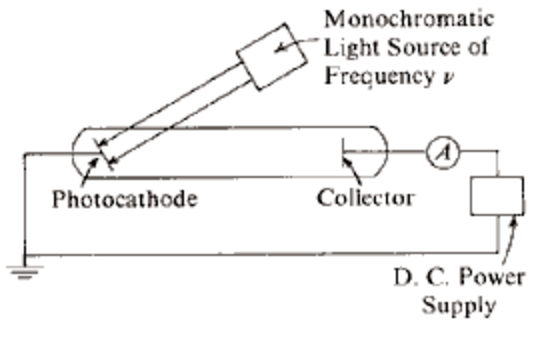
\includegraphics[width=\linewidth, height=50mm]{images/PhotoEE.png}
      \tiny (GRE 8677 \#31-33)
    \end{minipage}

\\ \hline

Photoelectric effect & Light is absorbed in quanta:  $E = h \nu$ \\
& \begin{minipage}{.4\textwidth}
 $|eV_0|= K_{max} = h \nu - W $ where $V_0$ is the stopping potential ($I=0$), $K_{max}$ is the maximum kinetic energy of an emitted electron, and $W$ is the work function of the metal. $W = h \nu_0$, where $\nu_0$ is the threshold frequency.
    \end{minipage}

\\ \hline
}

\Table{
\hline

Compton effect & 
\begin{minipage}{.3\textwidth}
      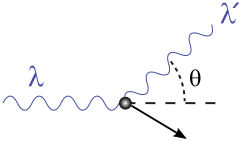
\includegraphics[width=\linewidth, height=25mm]{images/ComptonScat.png}
      \end{minipage}
      \\
      &
      \begin{minipage}{.6\textwidth}
       ``inelastic scattering of a photon by a charged particle, usually an electron. It results in a decrease in energy (increase in wavelength) of the photon (which may be an X ray or gamma ray photon)''
    \tiny \url{https://en.wikipedia.org/wiki/Compton_scattering}
    \end{minipage}
    \\
    &
    $\lambda' - \lambda = \dfrac{h}{m_e c} (1- \cos \theta)$
\\ \hline
}

\Table{
\hline

Franck-Hertz experiment & 
\begin{minipage}{.6\textwidth}
      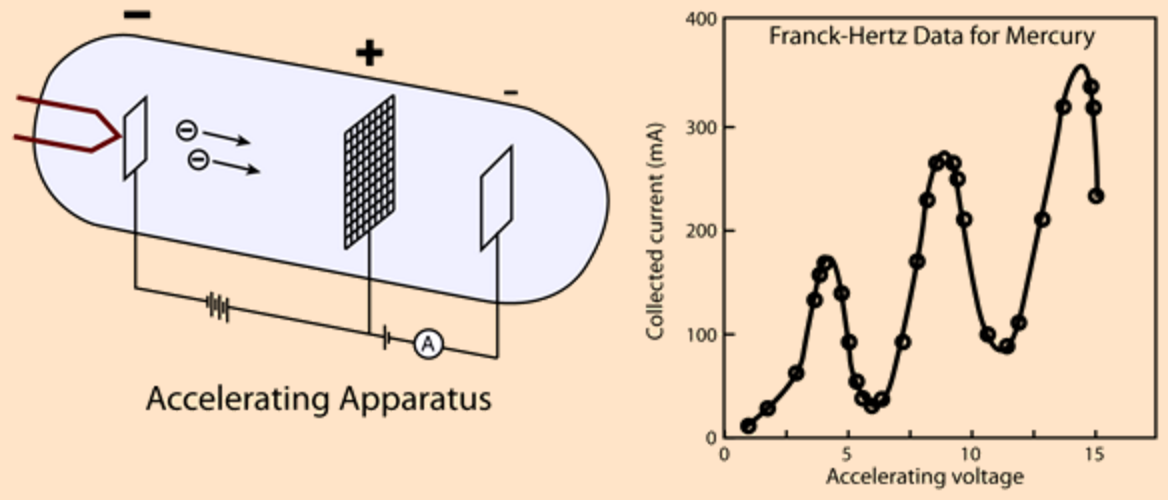
\includegraphics[width=\linewidth, height=45mm]{images/FranckHertz.png}
      \end{minipage}
      \\
      &
      \begin{minipage}{.6\textwidth}
       ``Electrons were accelerated by a voltage toward a positively charged grid in a glass envelope filled with \textbf{mercury vapor}. Past the grid was a collection plate held at a small negative voltage with respect to the grid. The values of accelerating voltage where the current dropped gave a measure of the energy necessary to force an electron to an excited state.'' \tiny \url{http://hyperphysics.phy-astr.gsu.edu/hbase/frhz.html}
    
    \end{minipage}
    
    
    
    
\\ \hline
}

\Table{
\hline

Angular momentum values & 
\MiniPg{.6}{
$l = 0,1,2,3,4,5,6,7,8$

$l = s,p,d,f,g,h,i,k,l$ 

For a given $n$, $l$ can take values up to $n-1$.

 Archaic: `s'harp, `p'rincipal, `d'iffuse, `f'undamental
}
\\ \hline
}

%%%%%%%%%%%%%%%%%%%%%%%%%%%%%%%%%%%%%%%%%

\subsection{Atomic structure} 
\Table{
\hline

State of an electron
&
\MiniPg{.7}{
\center

 $\psi(\bold{r}) \chi({\bold{s})}$
 \flushleft
 
Where $\psi$ is the spatial wave function and $\chi$ is the spinor.

Recall the composite spin states. The singlet state is antisymmetric and hence must be joined with a symmetric spatial function. Each triplet state is symmetric and requires a antisymmetric spatial function.

}

\\ \hline

Aufbau principle
&
\MiniPg{.7}{
      ``Hypothetically, electrons orbiting one or more atoms fill the lowest available energy levels before filling higher levels.''

\GraphicWHN{.6}{.5}{aufbau.png}

      \tiny \url{http://study.com/cimages/multimages/16/aufbau.png}
}

\\ \hline

Diagonal rule

&

\MiniPg{.7}{
\center
Orbitals are filled in order of increasing $n+l$ value.  $nl$:

\GraphicWHN{.25}{.2}{DiagonalOrdering.png}

\tiny \url{https://en.wikipedia.org/wiki/Aufbau_principle}

}

\\ \hline
}

%%%%%%

\Table{
\hline

\MiniPg{.3}{
Total angular momentum
}

&

$j = l + s$

\\ \hline

Hund's Rules

&

\begin{minipage}{.7\textwidth}
      I) Consistent with Pauli exclusion, the state with the highest total spin ($S$) has the lowest energy: $\uparrow S \equiv \downarrow E$
      
      II) For a given spin, the state with the highest total orbital angular momentum ($L$), consistent with overall antisymmetrization, will have the lowest energy. $\uparrow L \equiv \downarrow E$
      
      III) If a subshell ($n,l$) is no more than half-filled, then the lowest energy level has $J=|L-S|$; if it is more than half-filled, then $J = L + S$ has the lowest energy.
\end{minipage}

\\ \hline

Hieroglyphic & $^{2S+1}L_J$

\\ \hline
}

\Table{
\hline

First 36 configs. & \begin{minipage}{.3\textwidth}
      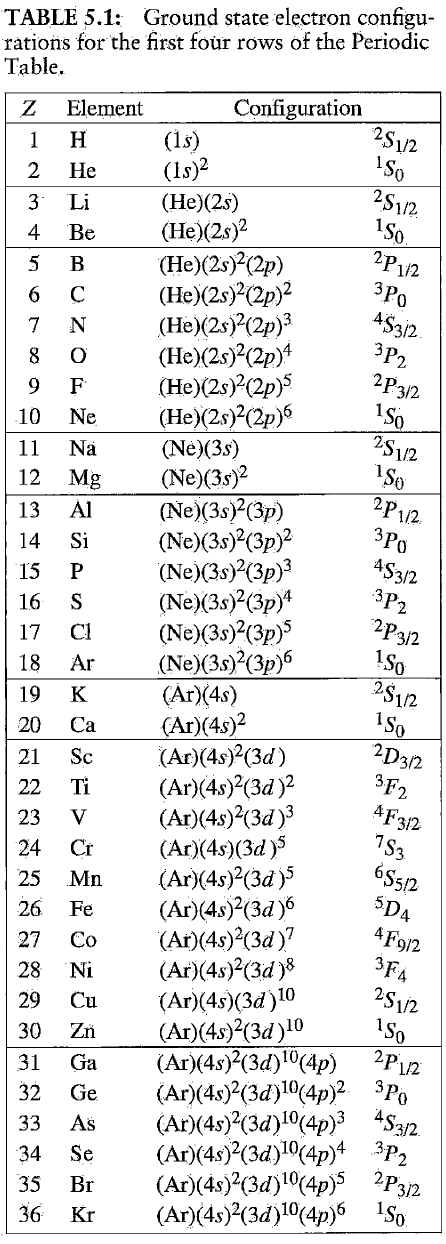
\includegraphics[width=\linewidth, height=125mm]{images/36Configs.png}
      \tiny Giffiths, \textit{Quantum}
    \end{minipage}

\\ \hline
}


%%%%%%%%%%%%%%%%%%%%%%%


\subsection{Atomic Spectra} 

\subsection{Selection rules}
\center
\begin{tabular}{|c|c|}
\hline

Selection rule for $m$ & No transitions occur unless $\Delta m = \pm1 \textrm{ or } 0$.

\\ \hline

Selection rule for $l$ & No transitions occur unless $\Delta l = \pm1$.
\\
&
\begin{minipage}{.6\textwidth}
      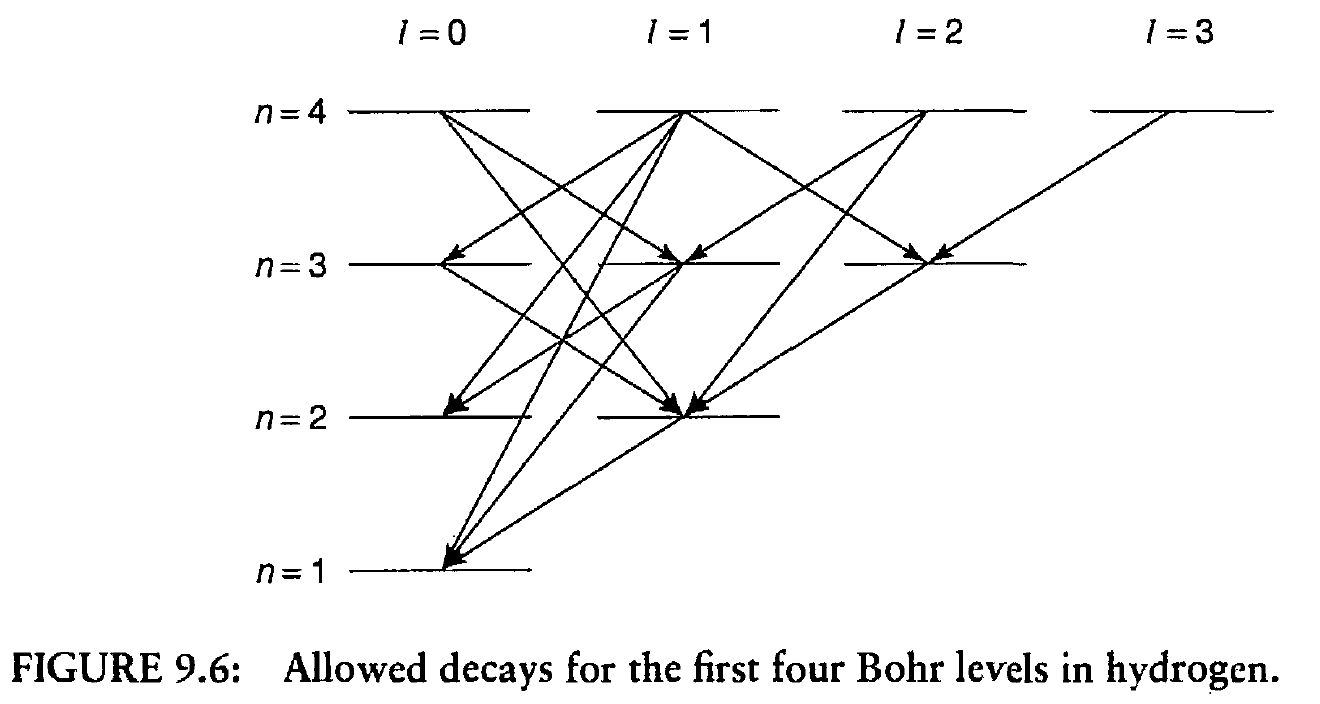
\includegraphics[width=\linewidth, height=50mm]{images/SelectionRuleL.png}
      \tiny Griffiths, \textit{Quantum Mechanics}
    \end{minipage}

\\ \hline
\end{tabular}
\flushleft

%%%%%%%%%%%%%%%%%%%%%%%%%%%%%%%%%%%%%%

\subsection{X-rays} 
\center

\begin{figure}[htbp]
    \begin{center}
	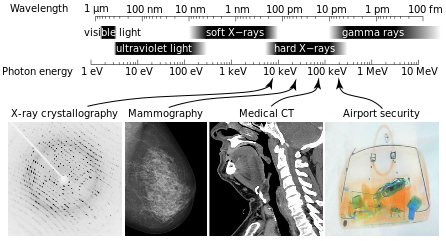
\includegraphics[width=110mm]{images/Xrays.png}
    \end{center}
    \linespread{1} 
	\caption[X-rays]{
	\tiny https://en.wikipedia.org/wiki/X-ray
	}
\label{xrays}
\end{figure}


%%%%

\begin{tabular}{|c|c|}
\hline

Xray transitions & \begin{minipage}{.5\textwidth}
      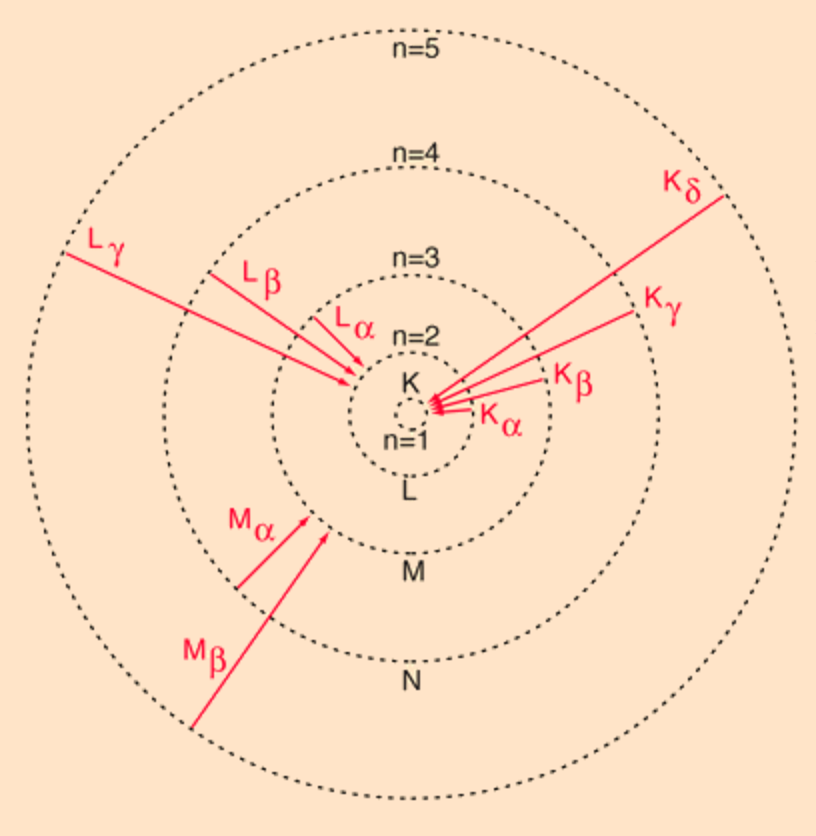
\includegraphics[width=\linewidth, height=80mm]{images/XrayTransitions.png}
      \tiny \url{http://hyperphysics.phy-astr.gsu.edu/hbase/quantum/xterm.html}
    \end{minipage}

\\ \hline

Moseley's Law & \\
\& description & 

\\ \hline
\end{tabular}
\flushleft

%%%%%%%%%%%%%%%%%%%%%%%%%%%%%%%%%%%%%%

\subsection{Atoms in electric and magnetic fields} 
